\documentclass[table]{beamer}
\usepackage[german]{babel}

\usepackage{tikz}
\usetikzlibrary{positioning,
                calc,
                decorations.pathreplacing,
                calligraphy}
\usepackage{tikzscale}
\usepackage{libertine}
\usepackage{pgf-pie}
\usepackage{hyperref}
\usepackage{booktabs}
\usepackage{diagbox}
\usepackage{xcolor}

\title{Versionskontrolle von Texten}
\subtitle{Git und GitHub}
\date{1. Februar 2024}

\begin{document}
    \frame{\titlepage}

    \begin{frame}
        \frametitle{Wichtige Quellen}
        \begin{itemize}
            \item git-scm.com
            \item docs.github.com/decorations
            \item code.visualstudio.com/docs/sourcecontrol/overview
        \end{itemize}
    \end{frame}

    \begin{frame}
        \frametitle{Ausgangslage}
        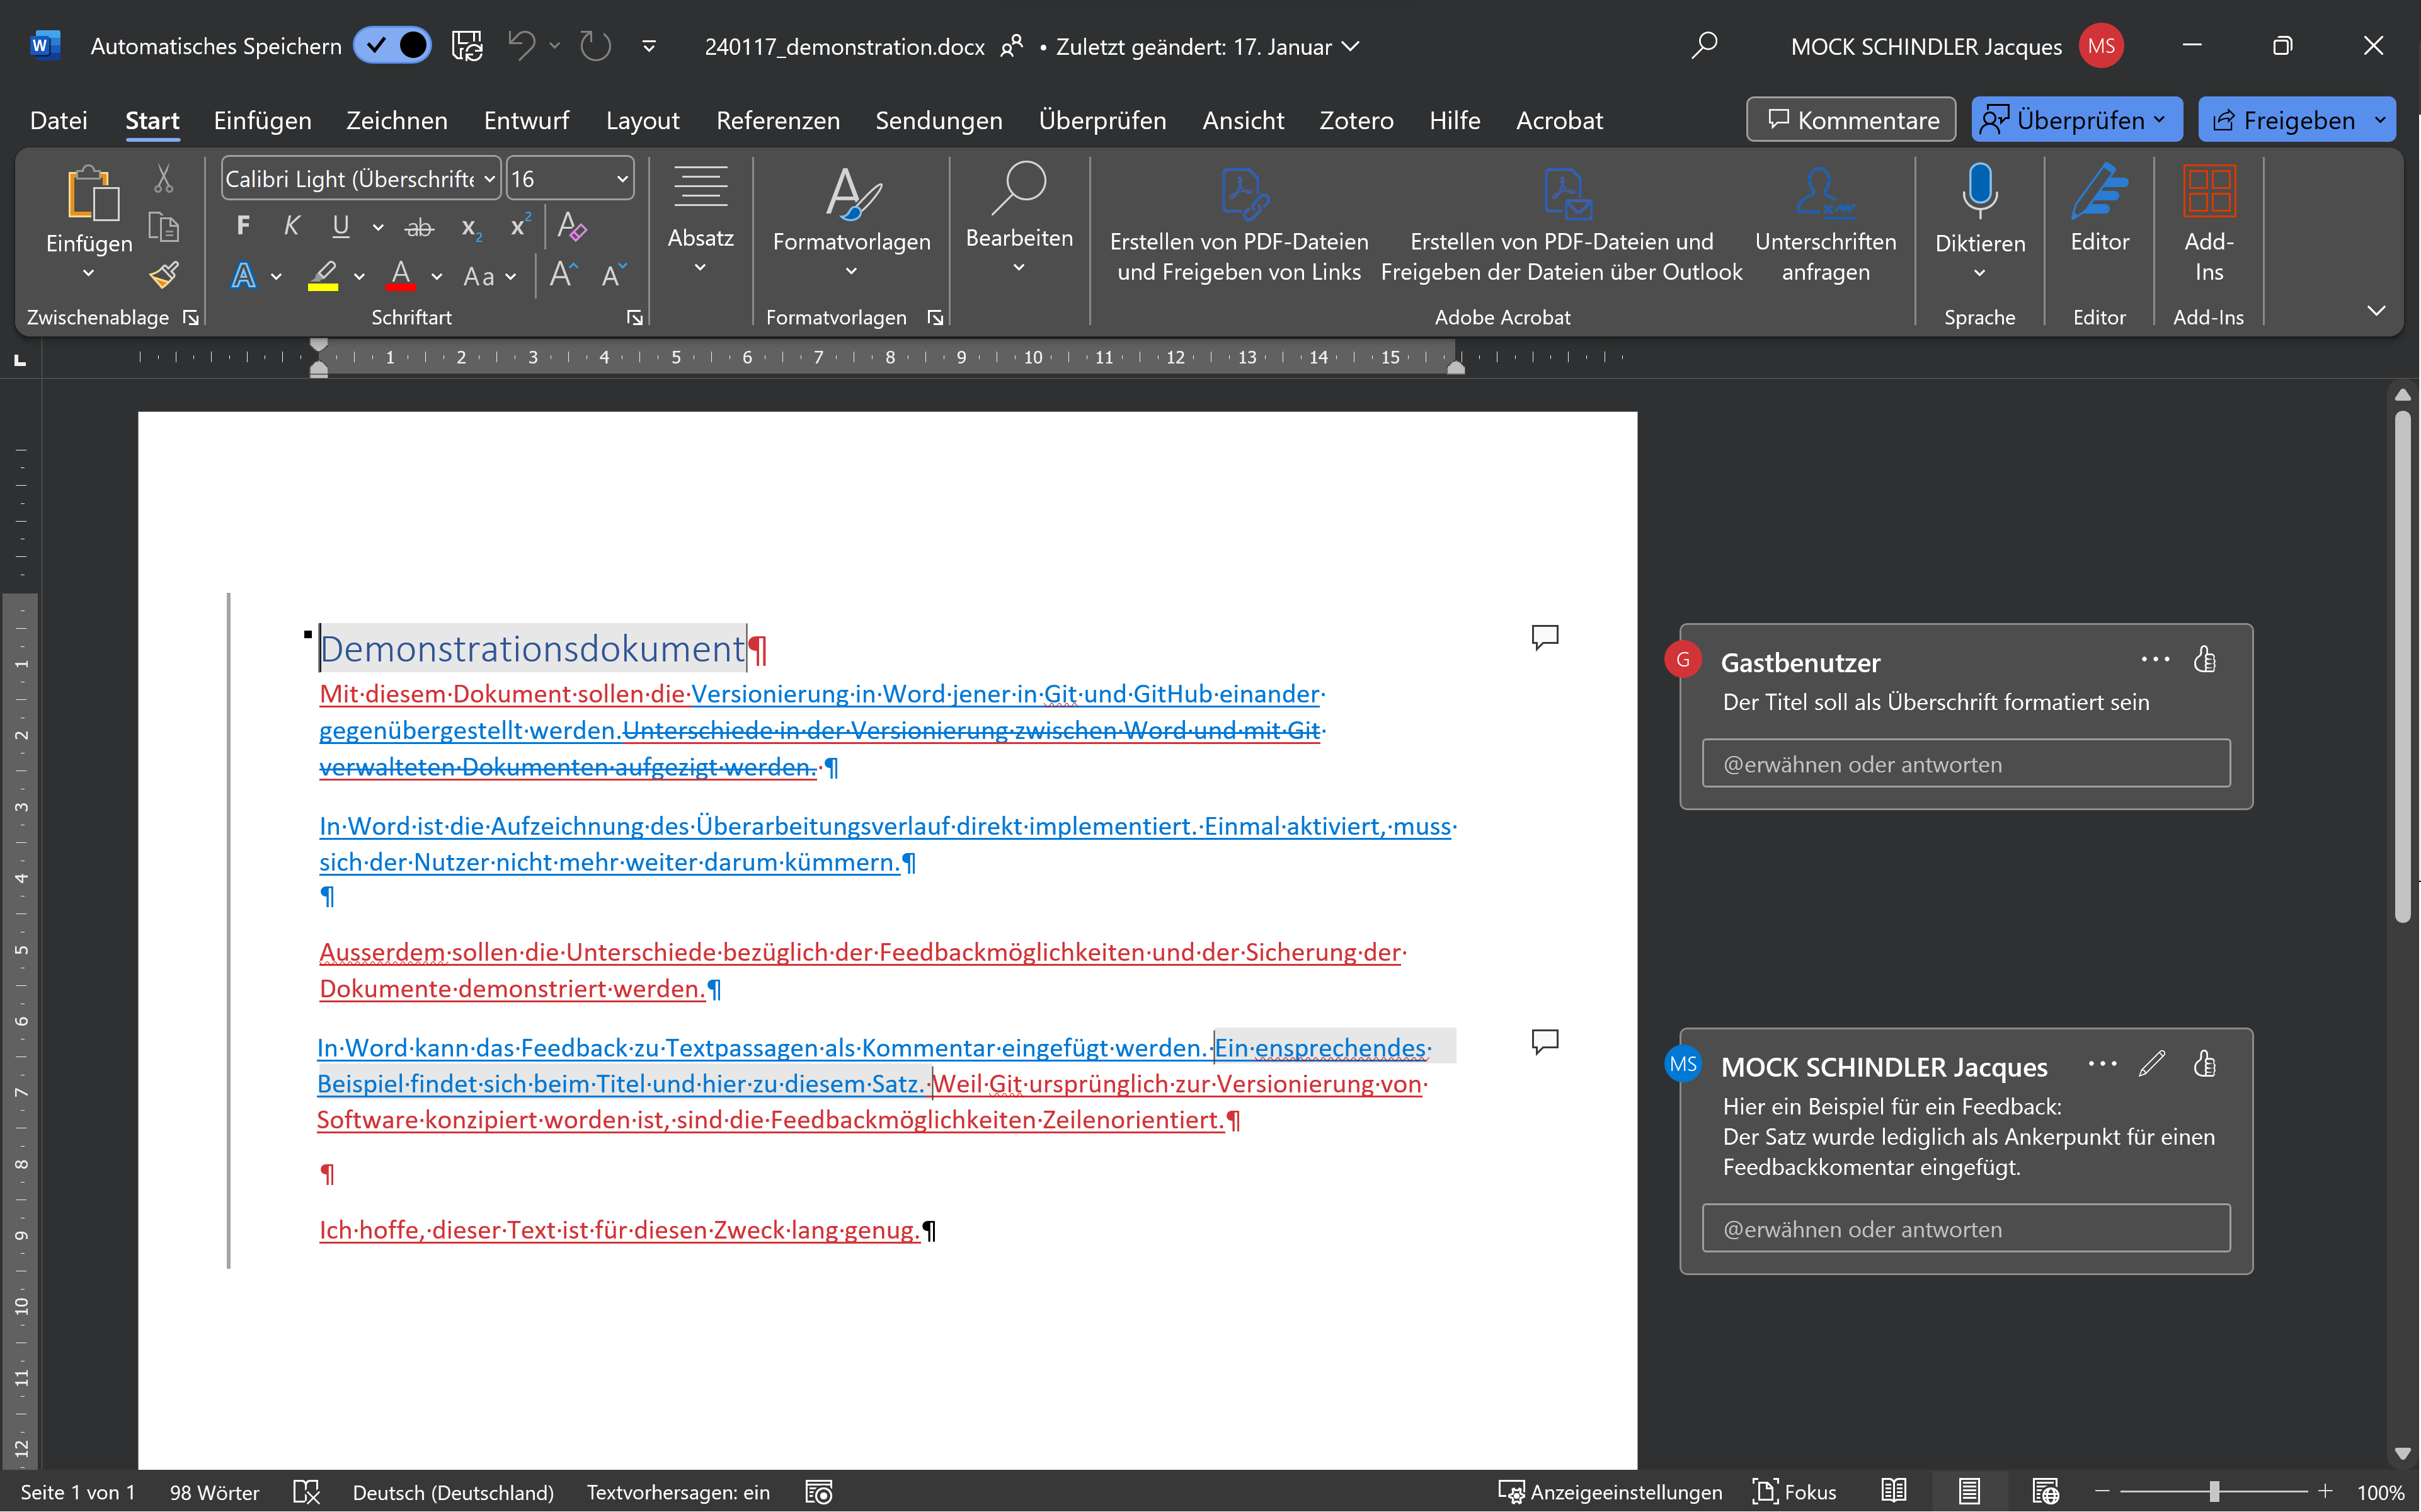
\includegraphics[width=\textwidth]{images/word_markup.png}
    \end{frame}

\end{document}
